%!TEX root = ../template.tex
%%%%%%%%%%%%%%%%%%%%%%%%%%%%%%%%%%%%%%%%%%%%%%%%%%%%%%%%%%%%%%%%%%%
%% chapter1.tex
%% NOVA thesis document file
%%
%% Chapter with introduction
%%%%%%%%%%%%%%%%%%%%%%%%%%%%%%%%%%%%%%%%%%%%%%%%%%%%%%%%%%%%%%%%%%%
\typeout{NT FILE chapter5.tex}%

\chapter{Proposed Work}

Finally, in the last section, we will outline our approach to tackle this project. We begin by describing and justifying our strategy, including the chosen approach and the technologies we will use. Then, we present our work plan, discussing ideas that may be useful for the development of the project. This section is divided into multiple iterations, which will span the duration of our thesis, including our evaluation plan, which will help ensure the success of the project.

\section{Technical Approach}
As mentioned in \ref{tab:problem_formulation}, the aim of this thesis is to design and implement an interactive tool to practice and evaluate logic exercises. The idea is to provide an online environment that will be easily accessible for everyone, where students can practice what they have learned in classes and be evaluated, while teachers can provide exercises for assessment. Unlike most online tools for learning logic, this one will pay special attention to the way it delivers assistance. We want to implement a system that is suitable for everyone, starting with the student who has no prior knowledge about logic to the expert who wants to improve his skills even more. 

To define our approach, we first need to select a set of exercises to implement. In logic, there are numerous types of exercises. According to professor Ricardo Gonçalves, who is currently the coordinator of the Computational Logic course at NOVA University Lisbon, the exercise where students show more difficulties is the \gls{ND} proofs. As explained in Chapter \ref{chap:prop-deduction}, this type of exercise requires significant exposure and practice to master. This exercise is also important, as it constitutes a significant part of the course at NOVA and is present in all tests and exams. Therefore, this tool will initially focus on implementing \gls{ND} exercises, but it will be designed to allow for future expansion. 

\gls{ND} proofs can be presented in many different ways, but we will work with a tree structure. These proofs can be done in both \gls{PL} and \gls{FOL}, so we will split this exercise into two different ones, with the second being an extension of the first, as it includes more rules and symbols. Besides that, we will have to establish a way to develop an effective and impactful feedback system that not only reports the students' mistakes but also provides mechanisms to assist them when they don't know how to progress.

To start with, we need to determine which architecture is most suitable for the development of a tool with these characteristics. The three-tier architecture is the one that best fits the requirements. Online tools scale significantly, especially this type of tool, where the number of simultaneous users is highly unpredictable~\cite{kircher_2025_the}. This architecture, by separating concerns into different layers, makes it easier to replicate and maintain. It also improves system reliability by facilitating the implementation of multiple levels of redundancy while providing ease of deployment. This architecture is divided into three tiers:

\textbf{Data (Database):} The data tier stores data in a persistent format. In our tool, this tier will be responsible for storing information about students, such as their proficiency level and their completed or in-progress proofs. It will also store exercises provided by teachers, as well as the grades for these exercises. For this, we will use a MySQL database, as it is relational, and the data we intend to store is also relational. Additionally, MySQL's ability to handle simultaneous operations from numerous users makes it suitable for online platforms with large user bases~\cite{gyordi_2016_a}. It also provides better support for transactions and data integrity, which is crucial for Systems used to evaluate students.
    

\textbf{Application (Server):} The application tier is the brain of the system. Not only is it responsible for communicating with the other tiers, but it also contains all the core functionality behind the tool. In this tier, we will implement the logic for the \gls{ND} exercises, the mechanism that manages users and provides access to different resources, and the system that generates the feedback. The technology that is ideal for us to use is the Spring Framework. Spring simplifies web application development, leading to increased productivity. It provides a decoupled way of developing web applications, making the process simpler through its various features~\cite{wali_2019_rapid}. Support for REST API\footnote{Representational State Transfer Application Programming Interface (REST API) is a popular architectural style for creating efficient and scalable web services~\cite{daruprasetyawan_2024_pengembangan}. It has become an important component of modern information technology ecosystems, facilitating interoperability among diverse Systems and platforms.} is one of the key features offered by Spring, facilitating communication with the presentation layer via HTTP requests and responses, enabling data exchange between the other two tiers of the application. Additionally, it offers built-in features to simplify communication with the database and to handle transactions.


\textbf{Presentation (Website):} The presentation tier is where users normally interact with the system, typically through a web page. Here, we will implement distinct environments for the different users that will be using the system. For this layer, we will use the React framework. It uses a declarative and object-oriented approach, which makes the code more intuitive and easier to maintain~\cite{madsen_a}. React's component-based architecture in hierarchy facilitates the creation of modular and reusable code by allowing developers to build complex pages from smaller, self-contained pieces. Another key feature of React is its ability to efficiently update user interfaces in response to state changes, which is a particularly useful feature when developing an interactive tool. Another technology that we will be using is Redux~\cite{freeman_2019_using}. It provides a centralized data store outside of the React component hierarchy, reducing system complexity by eliminating the need to pass state through multiple levels of components. This approach results in a more natural and organized application structure, making the state easier to manage and maintain.


\section{Work Plan}
An iterative model approach will guide the project's development process that focuses on continuous improvement. We will divide the implementation of this tool into three four iterations. The first iteration will comprise the basic features of an online tool with the \gls{ND} exercises. However, it will not include a feedback system. The second iteration will have a basic feedback system that will adjust according to the students proficiency. The third iteration will include an advanced feedback system that will be able to guide the student throughout the exercises. Each iteration will culminate in a final product that the students and teachers can test and use. The idea behind this is to always have a safe checkpoint throughout the development if something goes wrong. Since the feedback topics are harder to implement, we will keep them separated in two different iterations. Each iteration will involve conducting different evaluation processes to ensure the success of our project. In the final iteration, we will integrate our tool with the Moodle online e-learning platform. The sections below will present the different iterations that are divided into server and website implementations.

\subsection{First Iteration}
By the end of this first iteration, we aim to have a fully functional system that supports \gls{ND} exercises. Teachers will be able to provide new exercises in both languages, as well as view the answers and evaluations of the exercises. Students will be able to construct and validate their proofs. There won't be any detailed feedback in this iteration. The only feedback provided to the student will be a message indicating whether the proof is correct. This approach allows us to focus on the essential functionality of the system without the complexity of providing in-depth feedback at this stage. Future iterations may incorporate more detailed evaluations to enhance the learning experience.

\subsubsection{Server}
Our first task will be the implementation of a parser\footnote{A parser is a software component used in programming language processing that analyzes and interprets the structure of code or text according to a defined grammar~\cite{afroozeh_2015_one}.} for both \gls{PL} and \gls{FOL} expressions according to the grammar presented in \ref{chap:prop-syntax} and \ref{chap:fol-syntax}. After implementing the parsers, we will conduct a battery of tests to guarantee their correctness. 

Moreover, we will also implement a parser for \gls{ND} expressions. By defining a language to represent our own proofs, we can easily detect structural errors made by students. These steps are very important for setting up the feedback system because they can be used to give detailed help on syntax, like showing where mistakes happened and suggesting other ways to fix them. Similarly, the proof parser will undergo extensive testing.

The next step will be implementing the proof interpreter. This interpreter will take a well-formed proof as input and verify its correctness. It will begin by checking whether all derivations from the rules are correct. Then, it will verify the hypotheses and marks used in the proof, ensuring there are no unmarked leaves or missing hypotheses in the tree. Like the parsers, the interpreter will also go through extensive testing to ensure correctness.

Finally, we will implement a system to manage users and the system's exercises. There will be two types of users: students, who will have access to exercises and their grades, and teachers, who will create exercises and view grades of those exercises. This will require creating database tables to store user and exercise information, as well as defining the REST API endpoints that will interact with the webpage.

\subsubsection{Website}
After developing the server, we will move on to the implementation of the website. We will begin by defining the pages for students and teachers. 

Focusing only on the \gls{ND} proof environment, the goal is to create an intuitive and interactive platform for students to practice. To achieve this, proofs will be built using building blocks, with each block representing a sub-tree. The system will present users with a board on which they can add and edit blocks. Blocks can also be dragged and merged to form larger ones, resulting in bigger proofs solving the issue of directional flexibility discussed in Chapter \ref{chap:prop-deduction}. At this stage, since we don't have a feedback system implemented, we will provide the list of available rules as blocks, so the users don't need to define it manually. Figure \ref{img:building-blocks} shows a prototype of this environment.

\begin{figure}[htbp]
    \centering
    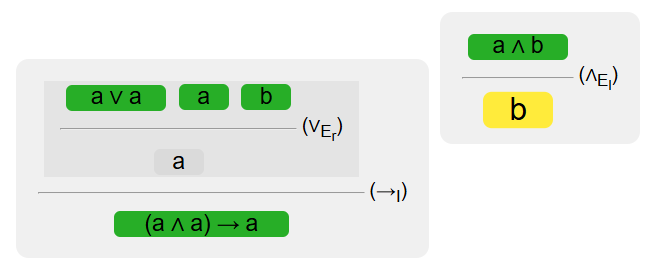
\includegraphics[width=0.5\linewidth]{prototype}
    \caption{Building blocks prototype.}
    \label{img:building-blocks}
\end{figure}

\subsection{Second Iteration}
By the end of this iteration, we aim to have a tool with a simplified feedback system, featuring different levels based on the students' proficiency. The system will identify both syntax and semantic errors in the submitted proofs.

\subsubsection{Server}
In this iteration, we will start implementing the feedback system, focusing on providing simple assistance. The system will provide balanced support to prevent students from relying solely on corrections. At the same time, it will make sure users have guidance so they know how to process it. 

To adjust the feedback to each student's level, we will assign a proficiency score, similar to what Iltis does. New users will start with a low score, which will increase as they complete exercises or decrease as they make mistakes. Higher scores will lead to more general feedback, while lower scores will provide more detailed help. To compute the score, we will categorize the exercises into different levels (e.g., easy, medium, and hard) as well as classify the mistakes (e.g., critical, moderate, and minor). This iteration will focus on syntax errors, which are related to the structure of expressions and proof grammar, and semantic errors, which concern the internal logic of the proof. Below are some examples of feedback for a syntactic error, based on proficiency levels:
\begin{itemize}
    \item \textbf{High proficiency:} "Your proof contains invalid expressions."
    \item \textbf{Intermediate proficiency:} "Expression \(a \lor b \to c\) is not valid."
    \item \textbf{Low proficiency:} "Expression \(a \lor b \to c\) is ambiguous. Consider including parentheses, possible correction: \((a \lor b) \to c\)."
\end{itemize}

\subsubsection{Website}
The feedback system will be fully integrated into the website and presented in a clear and interactive manner. The system will adapt dynamically based on the user's proficiency level. To achieve this, we will create distinct environments tailored to each user's proficiency level. For example, students with low scores will be presented with detailed information regarding the proof's current state, similarly to what some proof assistants do. Additionally, rules will be auto-filled to minimize cognitive load, and hypotheses will be automatically added to the list of hypotheses. As users progress and their proficiency increases, these assistive features will be gradually removed, requiring users to input rules manually and encouraging independent thinking. 
Another way to provide feedback is through visual changes in parts of the page. Visual feedback mechanisms, such as highlighting invalid expressions or marking tree segments with errors, will also be implemented to improve the user experience. Figure \ref{img:building-blocks-feedback} illustrates this feedback by highlighting the incorrect part of the proof.

\begin{figure}[htbp]
    \centering
    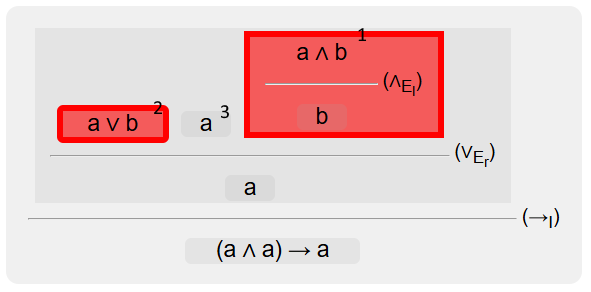
\includegraphics[width=0.5\linewidth]{prototype_feedback}
    \caption{Building blocks feedback prototype.}
    \label{img:building-blocks-feedback}
\end{figure}

\subsection{Third Iteration}
By the end of the third iteration, we will refine the feedback system, supporting advanced error detection and user interactions. We will introduce features such as displaying full proofs as possible solutions and providing hints about goals and the steps to follow during the proofs. Additionally, the interface will be polished, and the entire system will undergo extensive testing to ensure stability and reliability.

\subsubsection{Server}
In this iteration, we will start by defining the mechanism that will guide the student throughout the proof. Currently we found three possible ways to do that.

The first method involves the teacher providing a hidden solution while creating the exercise. This method encounters several challenges, including the inability to adjust to the student's solution and the constant need for a hidden solution.

Another solution is to use the Lean functional programming language~\cite{programming} to automate this process for us. We can define our own set of rules and use Aesop~\cite{leanprovercommunity_2021_github} for this purpose. While this approach seems straightforward, defining some of the rules from \gls{ND} (Annex \ref{ann:nd_rules}) and mapping our code to the Lean programming language can be challenging. Moreover, Aesop is not particularly powerful, as it can only find the more obvious proofs.

A final method is to develop an algorithm that attempts to find multiple solutions for the same proof, similar to what LOGAX does. However, since LOGAX focuses on a different domain of proofs and the rules provided by Bolotov's algorithm differ from the ones we will use, we need to create our own version of the algorithm. We have already developed some ideas on how to implement this algorithm, which are presented in Chapter \ref{tab:ad_algo}. By defining our own algorithm, we can create a fully controllable environment for the assistance system.

\subsubsection{Website}
Lastly, in this iteration, we will integrate advanced feedback into our webpage. This will involve implementing a system that highlights parts of the student's solution that could lead to dead ends or blocks that are irrelevant to the proof. Additionally, we will need to find an appropriate way to display feedback, either providing a full proof or partial hints in the form of sub-goals when the student gets stuck.

\subsection{Integration with Moodle}
The final iteration will be the integration of the tool with the Moodle online e-learning platform, allowing seamless access for students and teachers. This integration will enable features like automated grading and real-time tracking of student progress, ensuring a more interactive and efficient learning experience.

\subsection{Evaluation Plan}
To ensure the success of our project, we will conduct an evaluation process, focusing on key aspects such as correctness, usability, interactivity, and feedback effectiveness. We will use verification tests to ensure the system operates as intended and meets its specifications. We will use validation tests to assess the usability and interactivity of the tool, ensuring that it provides an intuitive experience for students. Additionally, we will evaluate the feedback mechanisms to ensure they provide meaningful and constructive assistance to users and to guarantee that they don't get stuck.

Verification tests will be conducted using the JUnit framework with extensive test cases. This will be done in the early stages of the project’s development, particularly when developing the parsers and the interpreter, and also immediately after each iteration to ensure the correctness of the system.

For the validation tests, we will focus on the usability and interactivity of the tool to guarantee that the system is user-friendly and has a low learning curve. To do this, we will organize testing sessions with participants of varying levels of proficiency in logic to interact with the system. During these sessions, we will observe how the users interact with the tool and assess their ability to use it efficiently. At the end of the sessions, we will conduct a survey to collect user feedback on the system’s usability, the clarity of the feedback provided, and their overall experience with the tool. This will help us identify areas for improvement and ensure that the tool meets the needs of the users. These tests will occur right after each iteration.


\section{Gantt Chart}
Below is the Gantt chart presenting all the stages previously mentioned in our plan.
\begin{figure}[htbp]
    \centering
    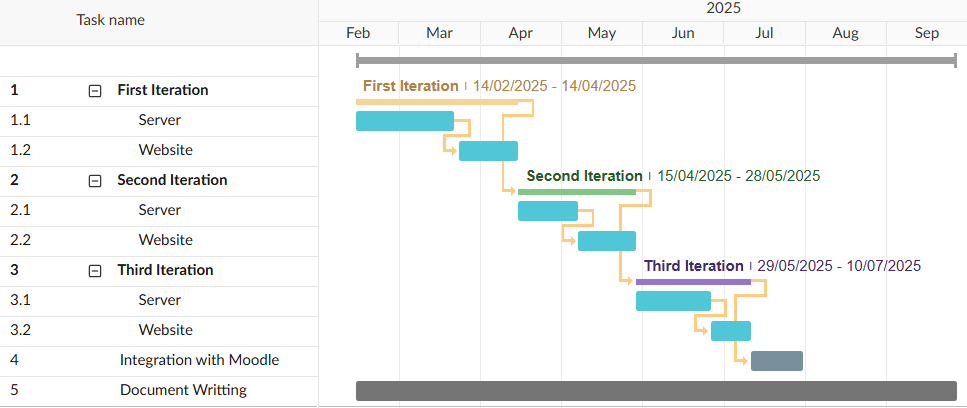
\includegraphics[width=1\linewidth]{gantt}
    \caption{Proposed Gantt Chart for the work plan.}
    \label{img:gantt}
\end{figure}